\documentclass{article}

\usepackage[T1]{fontenc}
\usepackage{svninfo}
\usepackage{graphicx}
\usepackage[round]{natbib}

\begin{document}

\bibliographystyle{abbrvnat}

\svnInfo $Id$

\newcommand{\dbatversion}{0.2}

\title{The Damped Bundle Adjustment Toolbox\\v\dbatversion{} for Matlab}
\author{Niclas B{\"o}rlin\\Department of Computing Science\\Ume{\aa}
  University\\niclas.borlin@cs.umu.se}
\date{\today}

\maketitle

\newpage

\tableofcontents

\newpage

\section{Introduction}

\subsection{Purpose}

Matlab toolbox with freely available code for bundle adjustment.
Intention to be state-of-the-art.

\subsection{Limitations}

What it can do.

What it cannot do.

\subsection{Legal}



\subsection{Scientific publications}

Refer to any of the papers...

\cite{Borlin2013:Bundle}
\cite{Borlin2013:Experiments}

\section{Installation}
\label{sec:install}

\begin{enumerate}
\item Download the package file {\tt
  \verb+dbat_+\dbatversion\verb+.zip+}.
\item Unpack the package into a directory \emph{dbat}.
\item \label{step:dbatInit}
Inside Matlab, do the following initialization:\\
\verb+cd dbat % the directory where you installed the files.+\\
\verb+dbatSetup % set paths, etc.+
\item Test the installation by executing \texttt{loadplotdemo}.
\item If \texttt{loadplotdemo} runs without errors and generates a
  figure with a camera network, the installation is ok.
\end{enumerate}

\section{Usage}

\subsection{Demos}

\subsubsection{loadplotdemo}

The \verb+loadplotdemo+ demo loads a modified Photomodeler text export
file of the 60-camera, 26000-point project used
in~\cite{Borlin2013:Bundle}. The camera network, as computed by
Photomodeler, is plotted with camera 1 aligned to the cardinal axes.
The result should look like Figure~\ref{fig:roma}. The figure is a
standard Matlab 3D figure and may e.g.\ be rotated or zoomed using the
camera toolbar.

\begin{figure}
  \centering
  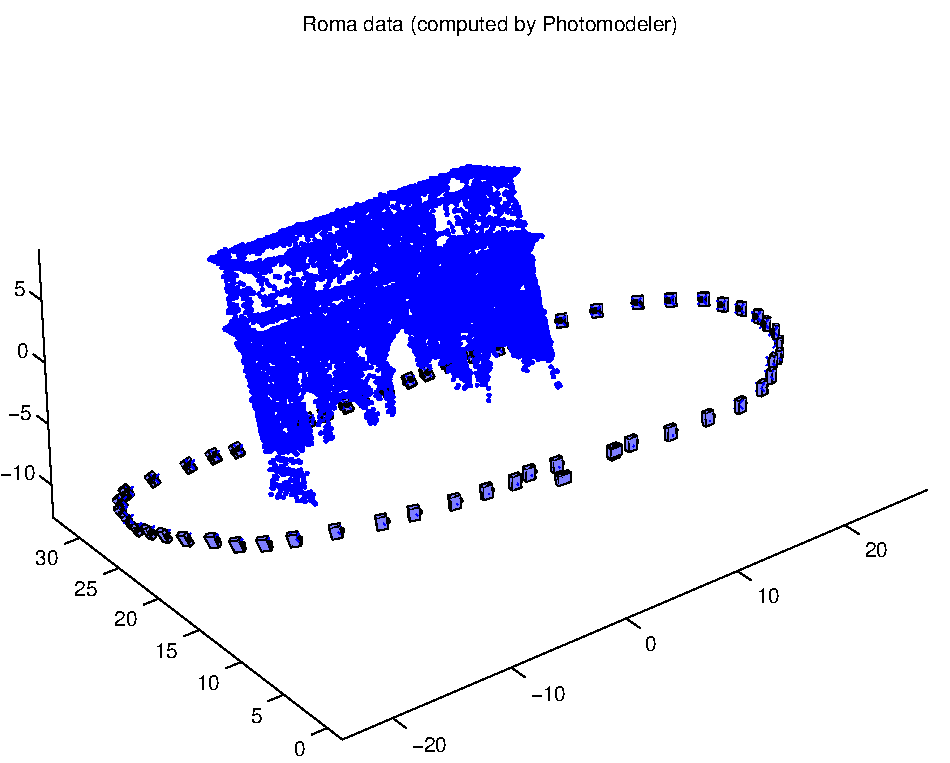
\includegraphics[width=0.6\hsize]{ill/roma}
  \caption{The figure generated by the \texttt{loadplotdemo} demo.}
  \label{fig:roma}
\end{figure}

\subsubsection{loadplotdemo2}
\label{sec:camcaldata}

The \verb+loadplotdemo2+ demo loads a modified Photomodeler text
export file of a 21-camera, 100-point camera calibration project. The
camera network, as computed by Photomodeler, is plotted and should
look like Figure~\ref{fig:camcalib}. The figure is a standard Matlab
3D figure and may e.g.\ be rotated or zoomed using the camera toolbar.

\begin{figure}
  \centering
  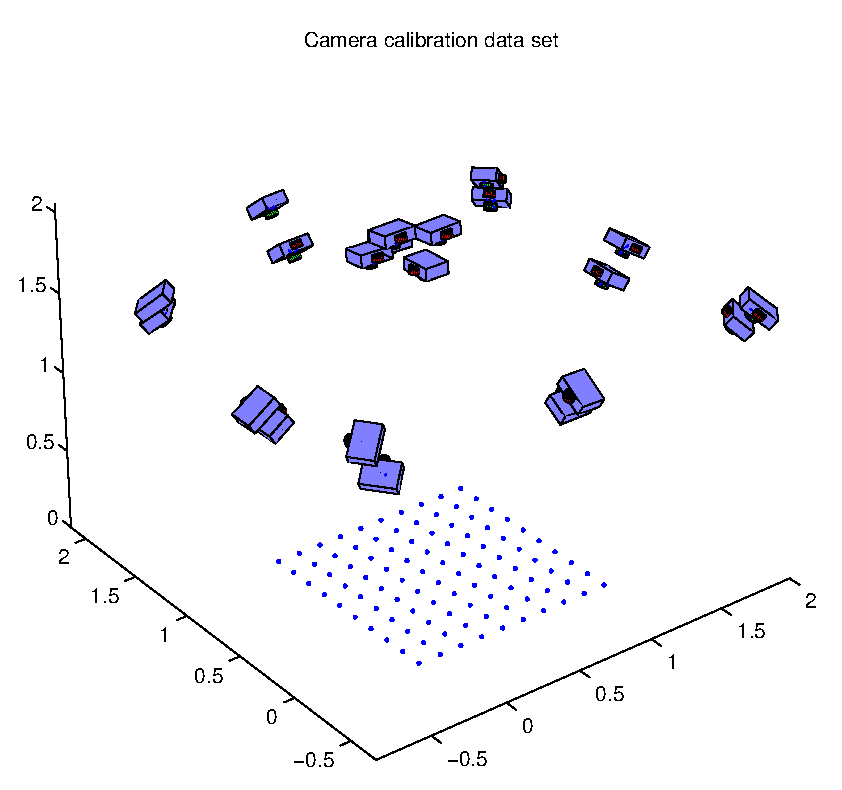
\includegraphics[width=0.6\hsize]{ill/ccam}
  \caption{The figure generated by the \texttt{loadplotdemo2} demo.}
  \label{fig:camcalib}
\end{figure}

\subsubsection{romabundledemo}

\subsubsection{camcaldemo}

The \verb+loadplotdemo2+ demo loads the camera calibration export file
from Section~\ref{sec:camcaldata} and runs a camera calibration. The
true focal length is used as initial value. The other values are set
to ``default'' values, e.g.\ the principal point is the center of the
sensor and all lens distortion parameters are zero.

The result is given

\end{description}
\subsection{Using your own data}

\subsubsection{Enabling text export from Photomodeler}
\label{sec:enableTextExport}.

Some versions of Photomodeler do not have the text file export option
enabled by default. In that case, follow the following steps to enable
it:
\begin{enumerate}
\item Right-click on the main window toolbar, select \emph{Customize toolbar...}.
\item In the \emph{Commands} tab, select the \emph{File} category.
\item Drag the \emph{Export Text File...} command to a toolbar of
  your choice.
\item Now you should be able to export your project as a text file by
  clicking on the \emph{Export Text File} button.
\end{enumerate}

\subsubsection{Export from Photomodeler}

To import a Photomodeler project into the toolbox, the following
steps are valid in Photomodeler Scanner 2012:

\begin{enumerate}
\item Export the project using \emph{Export Text File}. If the
  \emph{Export Text File} command is not available, follow the
  instructions in Section~\ref{sec:enableTextExport}.
\item After export, open the \emph{Project/Cameras...} dialog and
  select the camera that was used in your project.
\item Open the generated text file in a text editor.
  \begin{enumerate}
  \item On the 2nd line (usually reading \texttt{0.00005 20}), append
    the width and height in pixels of your images, e.g. to
    \texttt{0.000500 20 5616 3744}.
  \item Inspect the 4th line. For instance,
    the original data in \texttt{roma.txt} was (some trailing zeros removed):

    \texttt{24.3581 18.1143 12.0 35.96404 24.0 0.00022 -0.0 0.0 0.0 0.0}

    The values correspond to the following camera parameters:

    \texttt{focal pp\_x pp\_y format\_w format\_h K1 K2 K3 P1 P2}.

    Notice that most of the significant digits of K1--K3 were lost in
    the text export.
  \item Update the parameter values on the 4th line with values from
    the camera dialog \emph{for each parameter with a larger number of
      significant digits in the dialog}. This usually means all
    parameters except \texttt{format\_w}. In the \texttt{roma.txt}
    test case, the 4th line was modified to:

    \texttt{24.3581 18.1143 12 35.96404 24 2.174e-4 -1.518e-7 0 0 0}.

  \end{enumerate}
\end{enumerate}

\subsubsection{Loading into Matlab}

\begin{enumerate}
\item In matlab, run step~\ref{step:dbatInit} from
  Section~\ref{sec:install} if not already done.
\item \sloppy Set the variable \texttt{fName} to the text export file name \texttt{fName='c:/path/to/exported/file.txt';}, or
  select it using \texttt{[f,p]=uigetfile('*.txt'); fName=[f,p];}
\item Run the \texttt{loadplotdemo} script. A figure with your camera
  network, aligned with the first camera and rotated to have +Z 'up',
  should now have been generated.
\end{enumerate}

\bibliography{ref}

\appendix

\section{Camera model}

\end{document}
